\documentclass{report}
% \documentclass[oneside]{report}
% \documentclass[openany]{book}

\usepackage[T1]{fontenc}
\usepackage[utf8]{inputenc}
% \renewcommand{\familydefault}{\sfdefault}
% \usepackage{csquotes}
% \usepackage[croatian]{babel}
% \usepackage[fixlanguage]{babelbib}
\usepackage{amsfonts}
\usepackage{amssymb}
\usepackage{amsmath}
\usepackage{listings}
\lstset{
  basicstyle=\ttfamily,
  mathescape
}
\usepackage{tikz}
% \usepackage{circle}
\usepackage{geometry}
    \geometry{
        a4paper,
        total={150mm,237mm},
        left=30mm,
        top=30mm,
    }
\usepackage{biblatex}
\usepackage{cases}
\usepackage{float}
\usepackage{mathtools}
\usepackage{pdfpages}
% \usepackage{algorithm}
% \usepackage{algpseudocode}

\usepackage{tikz}
\usetikzlibrary{arrows}
\usetikzlibrary{shapes,arrows}
\usetikzlibrary{positioning,fit,calc}
\usetikzlibrary{shapes.geometric, arrows}
\addbibresource{bibliography/references.bib}

\newtheorem{theorem}{Theorem}[chapter]
\newtheorem{definition}{Definition}[chapter]
\newtheorem{lemma}{Lemma}[chapter]


\title{A Real-Time, Flexible Logging and Monitoring Infrastructure for MonPoly}
\author{Jonas Degelo}
\date{February 2023}

\begin{document}

\newcommand*{\Until}[1]{\,\mathcal{U}_{#1}\,}
\newcommand*{\Since}[1]{\,\mathcal{S}_{#1}\,}
\newcommand*{\Next}[1]{\tikz\draw[] (0,0) circle (.8ex);_{#1}}
% \newcommand{\Next}{\Circle}
\newcommand*{\Previous}[1]{\tikz\draw[fill] (0,0) circle (.8ex);_{#1}}
% \newcommand{\Previous}{\Circle[f]}
\newcommand*{\Eventually}[1]{\lozenge_{#1}}
\newcommand*{\Once}[1]{\blacklozenge_{#1}}
\newcommand*{\Always}[1]{\square_{#1}}
\newcommand*{\Historically}[1]{\blacksquare_{#1}}
\newcommand*{\Fregex}[1]{\vartriangleright_{#1}}
\newcommand*{\Pregex}[1]{\blacktriangleleft_{#1}}

\newcommand*{\RI}{\operatorname{RI}}
\newcommand*{\RIr}{\operatorname{RI}_{\text{reg}}}
\newcommand*{\ERI}{\operatorname{ERI}}
\newcommand*{\ERIr}{\operatorname{ERI}_{\text{reg}}}

\newcommand*{\filter}{\operatorname{filter}}

\newcommand*{\Cupmerge}{\,\ddot{\Cup}\,}
\newcommand*{\Cupext}{\,\dot{\Cup}\,}
\newcommand*{\oplusext}{\,\dot{\oplus}\,}

\newcommand{\keys}{\operatorname{keys}}

\newcommand{\inveri}{\operatorname{inverseERI}}
\newcommand{\zeroeri}{\operatorname{zeroERI}}



\begin{titlepage}
    \begin{center}
        \vspace*{1cm}
        \Huge
        \textbf{A Real-Time, Flexible Logging and Monitoring Infrastructure for MonPoly} \\
        \vspace{0.5cm}
        \LARGE
        \vspace{1.5cm}
        \textbf{Jonas Degelo} \\
        \vspace{1.5cm}
        Supervisor: \\
        François Hublet \\

        Professor: \\
        Prof. Dr. David Basin
        \vfill
        Bachelor's Thesis \\
        \vspace{0.8cm}
        \Large
        Information Security Group\\
        Department of Computer Science\\
        ETH Zürich\\
        February 2023
    \end{center}
\end{titlepage}

\tableofcontents
\newpage

\section{Introduction}

This project concerns itself with the problem of runtime verification.

\cite{Basin2016}

\section{Background}

\subsection{Metric First-Order Temporal Logic}
As mentioned in the introduction, Metric First-Order Temporal Logic (MFOTL) \cite{Basin2008, Basin2015, Chomicki1995} is used as a policy specification language by MonPoly.
Here we give a quick overview of MFOTL.
MFOTL is well suited to express a variety of policies one might want to monitor.
It combines First Order Logic (FOL) with metric temporal operators.
FOL provides us with common logic operators like $\land$ ("and"), $\lor$ ("or"), and $\neg$ ("not") as well as quantifiers $\forall$ ("for all") and $\exists$ ("exists").
The metric temporal operators in MFOTL are $\Until_I$ ("until"), $\Since_I$ ("since"), $\Previous_I$ ("previous"), and $\Next_I$ ("next").
These operators can be used to construct further syntactic sugar operators such as $\Once_I$ ("once"), $\Eventually_I$ ("eventually"), $\Always_I$ ("always"), and $\Historically_I$ ("historically").
See Basin et al. 2015 \cite{Basin2015} for the concrete derivations of these additional operators.
The metric aspect of these operators is the interval $I$ they are bound by.
This interval denotes a time frame in which the formula needs to be satisfied.

Basin et al. 2008 \cite{Basin2008} define the syntax and semantics of MFOTL.


Metric First-Order \textit{Dynamic} Logic (MFODL) \cite{Basin2020} is an even more expressive specification language than MFOTL.
MFODL introduces the notion of regular expressions.
For an exact definition of these regular expressions and the two new operators they introduce see figure 4 of Basin et al. 2020 \cite{Basin2020}.
Similarly to how $\Once_I$, $\Eventually_I$, $\Always$, and $\Historically$ can be derived from the four core operators $\Until_I$, $\Since_I$, $\Previous_I$, and $\Next_I$, these core operators could theoretically be replaced by the two new regular expression operators.
The exact conversion can also be seen in Basin et al. 2020 \cite{Basin2020}.
In practice, it is often useful to keep the basic temporal operators as we can apply specialized optimizations to them that cannot be done with regular expressions.

Basin et al. 2015 \cite{Basin2015aggregations} extends MFOTL with aggregations.
Aggregation operations like SUM are commonly seen in database contexts.
When considering an example like a monthly spending limit for a credit card it becomes clear how aggregations can be useful in policy monitoring.


\subsection{MonPoly}
MonPoly \cite{Basin2017} is a policy monitoring tool written in OCaml that supports MFOTL with aggregations and in its newest iterations it also has support for MFODL.
MonPoly can monitor a fragment of MFOTL/MFODL where all future operators must be bounded.
One major exception to that rule is an (implicit) always operator around the desired policy.

Let's return to the social media example from the introduction and look at how we would go about monitoring that policy with MonPoly.
We recall our description in words:
    "If a user's location data is accessed and the purpose of the access is for tailoring advertisements, the user must have previously given permission for there location data to be used for advertising purposes"
In MonPoly a policy is tied to a signature.
A signature can be compared with a database schema and describes the arity and types of possible events.
So let's consider a possible signature for our example: 

\begin{verbatim}
loc_accessed(user_id: int, purpose: string)
perm_granted(user_id: int)
perm_revoked(user_id: int)
\end{verbatim}

This is a basic signature with 3 predicates.
The first one means that a users location data has been used for a specified purpose.
The last two events get triggered when a user either grants or revokes permission for their location data to be used for advertising purposes.
Let's now define the policy in a formal manner.
\begin{align*}
    \Always (\texttt{loc\_accessed(i, "advertising")}
    \implies (\Once_{[0,\infty)} &\texttt{perm\_granted(i)} \\
         \land  \neg (\texttt{perm\_revoked(i)} \Since_{[0,\infty)} 
            &\texttt{perm\_granted(i)})))
\end{align*}

For MonPoly we first get rid of the surrounding $\Always$, because MonPoly implicitly adds an always-operator around any policy.
The remaining formula in MonPoly syntax is the following:

\begin{verbatim}
loc_accessed(i, "advertising")
IMPLIES 
(
    (ONCE[0,*) perm_granted(i)) 
    AND 
    (NOT (perm_revoked(i) SINCE[0,*) perm_granted(i)))
)
\end{verbatim}

While MonPoly cannot actually monitor this formula directly, it can monitor the negation of this formula.
For this on can use the \texttt{-negate} flag when running MonPoly.

\subsection{Time Series Databases}

Time series databases are a class of databases optimized for timestamped data.
For example, they optimize for data retrieval within a certain time range.
With the advance of internet of things devices with built-in sensors time series databases are experiencing explosive growth.
And as we have established they happen to fit well with our monitoring goals.
There are many different options of time series databases available.
We were looking for something with good performance, good support for tables of data, and good usability.
We have opted for QuestDB \cite{questdb}.

QuestDB uses a column-based storage model \cite{questdb-storage-model}.
It supports the PostgreSQL wire protocol \cite{questdb-postgres-wire} for querying and inserting data.
% TODO describe protocol
It further provides a REST API and has a web console for both inserting and querying data.
For best performance it supports the InfluxDB Line Protocol \cite{questdb-influx-db-line-protocol} with client libraries for most popular modern programming languages.
% TODO describe protocol
QuestDB itself is written in Java, open source, and licensed under the Apache 2.0 license.
% TODO describe addition of timestamp in rows
% TODO describe form of queries
 



\section{Architecture}

In this section we introduce the general architecture of our wrapper for MonPoly.
A more in depth look at the specific technical implementation will be provided in the implementation section.
In general, we have three components for this project.
On one hand we have the MonPoly with a few extensions.
On the other hand is QuestDB.
Our wrapper acts as the glue between the two.
In addition the wrapper also provides a new interface to MonPoly in the form of a REST API.

% TODO insert diagram of different components
\tikzset{block/.style={draw, thick, text width=3cm, minimum height=1.5cm, align=center},   
% the align command is used to align the block diagram at the center  
% the height command adjust the height of the block diagram  
% here block diagram refers to the whole diagram, not the single block  
% the thick command here signifies the border of all the blocks used inside the block diagram. You can change it to thin command if you want the thin edge of the blocks  
line/.style={-latex}   % the lesser the width the greater will be the diagram window  
}  

\begin{tikzpicture}[node distance=2.5cm,auto,>=latex']
    \node[block] (a) {Wrapper};  
    \node[block,right=of a] (b) at ([yshift=1cm]$(a)$) {MonPoly};
    % you can use as many blocks by specifying the name and alphabets  
    \node[block,right=of a] (c) at ([yshift=-1cm]$(a)$){Questdb};  
    % the yshift here specifies the shift in the position of the point on the y-axis. You can change the location according to the requirements.  
    % the value mentioned is the distance from (b) to (c). If the value is 0.5, then the block will be at the center of (b) and (c).  

    \draw[line] (a)--(b);  
    \draw[line] (a)--(c);
\end{tikzpicture}



\subsection{Wrapper}

The wrapper can be run directly on a system with MonPoly installed.
The alternative and more portable way to run it is with a docker container.
To interact with the wrapper a user can use the provided REST API by sending web requests.

The wrapper runs MonPoly as a subprocess and handles all interactions with MonPoly itself.
Incoming events are first parsed and checked on some major formatting errors.
When the formatting is deemed acceptable the events get forwarded to MonPoly on a per time stamp basis.
If MonPoly reports an issue with a certain time stamp, either it is out of order or one event at that timestamp does not comply with the given signature, this time stamp gets ignored by MonPoly, and in turn the wrapper discards it as well.
If no issue is detected with a timestamp all events in at that timestamp get forwarded to the database.

\tikzstyle{startstop} = [rectangle, rounded corners, 
minimum width=3cm, 
minimum height=1cm,
text centered, 
draw=black]
% fill=red!30]

\tikzstyle{io} = [trapezium, 
trapezium stretches=true, % A later addition
trapezium left angle=70, 
trapezium right angle=110, 
minimum width=3cm, 
minimum height=1cm, text centered, 
draw=black]
% , fill=blue!30]

\tikzstyle{process} = [rectangle, 
minimum width=3cm, 
minimum height=1cm, 
text centered, 
text width=3cm, 
draw=black] 
% fill=orange!30]

\tikzstyle{decision} = [diamond, 
minimum width=2cm, 
minimum height=1cm, 
text centered, 
text width=3cm,
draw=black]
% fill=green!30]
\tikzstyle{arrow} = [thick,->,>=stealth]

\begin{tikzpicture}[node distance=2cm]

% \node (start) [startstop] {Start};
% \node (in1) [io, below of=start] {Events get sent to wrapper};
\node (in1) [io] {Events get sent to wrapper};
\node (pro1) [process, below of=in1] {Wrapper checks JSON formatting};
\node (dec1) [decision, below of=pro1, yshift=-1.5cm] {JSON formatting correct?};

\node (pro2a) [process, below of=dec1, yshift=-2cm] {Convert JSON input to list of MonPoly style log strings for each time point};
\node (pro2b) [io, right of=dec1, xshift=3.2cm] {Abort and report issue to user};
\node (pro3) [process, below of=pro2a] {Send next time point to MonPoly};
\node (dec2) [decision, below of=pro3, yshift=-2cm] {Time point in order and predicates comply with signature?};
% \node (stop) [startstop, below of=pro3]{Stop};

% \draw [arrow] (start) -- (in1);
\draw [arrow] (in1) -- (pro1);
\draw [arrow] (pro1) -- (dec1);
\draw [arrow] (dec1) -- node[anchor=east] {yes} (pro2a);
\draw [arrow] (dec1) -- node[anchor=south] {no} (pro2b);
\draw [arrow] (pro2a) -- (pro3);
\draw [arrow] (pro3) -- (dec2);

\end{tikzpicture}

\subsection{Policy Change}

This first version of a policy change functions by stopping the current monitor and starting a new one.
When starting the new monitor we want to restore the state of the old one.
We do this by querying old events from our database.
But we do not simply query for the entirety of the database.
We make two optimizations.
First we use relative intervals and second we make use of constant values.
For each predicate occurring in a formula we look for constant attributes in its occurrences.
For every predicate and its potential occurrences with different constant values we then compute an over approximation of the relative interval.
We use this information to create a SQL query that only queries the constant values combined with the interval.
This way we minimize the amount of data that the new monitor has to read and process.


\chapter{Algorithms}

\section{Policy Change}
This section gives a high level view of our policy change method.
The individual parts of the policy change will be explained in the following sections of this chapter.
We have a running instance of MonPoly monitoring some policy.
The user asks the wrapper to monitor a new policy.
The wrapper checks the monitorability of the new policy against the existing policy.
If it is not monitorable the wrapper keeps the current instance of MonPoly running and reports the issue with the new policy to the user.
Otherwise the wrapper uses MonPoly to get the extended relative intervals of the new policy.
Then these extended relative intervals get converted to SQL queries and the wrapper runs these queries on QuestDB.
The response from QuestDB gets converted into a MonPoly log file.
Next the wrapper stops the current iteration of MonPoly and starts a new one that first reads the created log file.
At this point the policy change is done, and the wrapper can continue with its normal operation.

% \textit{TODO write some pseudo code here}


\section{Relative Intervals}

First we append the definition of relative intervals from Basin et al. \cite{Basin2016} to include all operators currently supported by MonPoly.
Namely we add definitions for the MFODL operators.
Intervals are defined over $\mathbb{Z}$ and can either be open or closed.
The operators $\oplus$ and $\Cup$ are defined the same way as in Basin et al. \cite{Basin2016}.
Let $I$ and $J$ be some arbitrary intervals then $I \oplus J := \{i+j \mid i \in I \text{ and } j \in J\}$ and $I \Cup J$ is the smallest interval containing all values in both $I$ and $J$.

\begin{equation*}
    \RI(\varphi) =
    \begin{cases}
        \{0\}     & \text{if $\varphi$ is an an atomic formula,} \\ 
        \RI(\psi) & \text{if $\varphi$ is of the form $\neg \psi$, 
                            $\exists x.\psi$,} \\ &\text{or $\forall x.\psi$,} \\
        \RI(\psi) \Cup \RI(\chi) & \text{if $\varphi$ is of the form $\psi \lor \chi, or
                                         \psi \land \chi$,} \\
        (-b,0] \Cup ((-b,-a] \oplus \RI(\psi)) & \text{if $\varphi$ is of the form $\Previous_{[a,b)}\psi$,} \\
        [0,b) \Cup ([a,b) \oplus \RI(\psi)) & \text{if $\varphi$ is of the form $\Next_{[a,b)}$,}\\
        (-b,0] \Cup ((-b,0] \oplus \RI(\psi)) \Cup ((-b,-a] \oplus \RI(\chi)) & \text{if $\varphi$ is of the form $\psi \Since_{[a,b)} \chi$,} \\
        [0,b) \Cup ([0,b) \oplus \RI(\psi)) \Cup ([a,b) \oplus \RI(\chi)) & \text{if $\varphi$ is of the form $\psi \Until_{[a,b)} \chi$,} \\
        [0,b) \Cup ([0,b) \oplus \RIr(\rho)) & \text{if $\varphi$ is of the form $\Fregex_{[a,b)} \rho$, and}\\
        (-b,0] \Cup ((-b,0] \oplus \RIr(\rho)) & \text{if $\varphi$ is of the form $\Pregex_{[a,b)} \rho$.}\\
    \end{cases}
\end{equation*}

We recursively define the relative interval of regular expressions as seen in Basin et al. \cite{Basin2020} in the following way.

\begin{equation*}
    \RIr(\rho) =
    \begin{cases}
        \{0\} & \text{if $\rho$ is of the form $\star^k$,} \\
        \RI(\varphi) & \text{if $\rho$ is of the form $\varphi?$,} \\
        \RIr(\sigma) \Cup \RIr(\tau) & \text{if $\rho$ is of the form $\sigma + \tau$ or $\sigma \cdot \tau$, and} \\
        \RIr(\sigma) & \text{if $\rho$ is of the form $\sigma^*$.}

    \end{cases}
\end{equation*}

\subsection{Correctness}
% TODO
Basin et al. \cite{Basin2016} provides an intuition for why the definition of $\RI$ is correct for the MFOTL operators.
Here we provide the same for the added MFODL \cite{Basin2020} operators and the regular expressions.

The definition of relative intervals is correct if any formula $\varphi$ evaluated on a trace $\sigma$ has the same truth value as evaluated on a trace $\sigma'$ that is a filtered version of $\sigma$ based on $\RI(\varphi)$.
Let $\RI(\varphi) = [a,b)$ where $a,b \in \mathbb{Z}, \, a \leq 0, \, b > 0$.
Given that no future events can be extracted from a trace as they have not happened yet, the extracted trace $\sigma'$ only contains time points with time stamps that are in the interval $[a,0]$.
Formally $\sigma' = \{x \mid x \in \sigma \text{ and } x.ts \in [a,0]\}$, where $x.ts$ denotes the time stamp of $x$.

The future match operator $\Fregex_I \rho$ depends on the relative interval of $\rho$ shifted by the interval $I$.
Similarly the past match operator $\Pregex_I \rho$ depends on the relative interval of $\rho$ shifted by the inverted interval $I$.
The interpretation of the relative intervals for regular expressions is a bit different from that of a formula.
Its relevance is the amount that the "parent" interval of a past or future match operator needs to be shifted by.
The wildcard operator $\star^k$ doesn't have any interval information attached.
The parameter $k$ refers to a number of timepoints, but not directly to time stamps.
The test operator $\varphi ?$ is more involved.
It evaluates a formula $\varphi$ which of course has a regular relative interval.
Depending on which match operator is used we want to evaluate $\varphi$ with any starting point inside the specified past or future interval.




\section{Relative Interval Extension}

This idea of relative intervals can already filter an existing trace down to a much smaller one by removing events that are unnecessary for the evaluation of a given policy.
We expand on this by creating and using a data structure that allows us to select an even smaller sub trace with the same effect of not changing the truth value of the policy.

First we move from one relative interval for an entire policy to one relative interval per predicate occurring in a policy.
We break this down further.
Every predicate comes with a number of attributes as defined in the signature.
Some attributes are potentially constant.
Looking back at our example from earlier, \texttt{"advertising"} is one such constant attribute in the predicate \texttt{loc\_accessed}.

\begin{verbatim}
loc_accessed(i, "advertising") 
IMPLIES 
(
    (ONCE[0,*) perm_granted(i)) 
    AND 
    (NOT (perm_revoked(i) SINCE[0,*) perm_granted(i)))
)
\end{verbatim}

This means any occurrence of the predicate \texttt{loc\_accessed} where the second attribute is not \texttt{"advertising"}, has no influence on our policy and is therefore not needed in a potential sub trace.
We check every predicate in our policy for constant attributes.
Then we take the set of different arrangements of constant and variable attributes per predicate.
We call one such arrangement a mask.
Each mask has its own relative interval.
For our example the masks with their corresponding relative intervals are the following.

\begin{verbatim}
loc_accessed(*,"advertising") -> [0,0]
perm_granted(*) -> (*,0]
perm_revoked(*) -> (*,0]
\end{verbatim}

A \texttt{*} in the attributes denotes a variable value.
In larger formulas there can be multiple different masks per predicate.

We use a doubly nested map data structure to store the predicates with there masks and relative intervals and call such a structure the extended relative intervals of a formula.
On the first level the keys are predicate names and values are maps from masks to intervals.
On this data structure we define the operators $\Cupmerge$, $\Cupext$ and $\oplusext$.
Let $m$ and $n$ be two extended relative intervals and $i$ a positive interval, then 
\begin{align*}
    m \Cupmerge n = 
        & \{ p(l) \rightarrow (i \Cup j) \mid 
            p(l) \rightarrow i \in m \text{ and } 
            p(l) \rightarrow j \in n \} \\
        & \cup \{p(l) \rightarrow i \mid  
            (p(l) \rightarrow i \in m \text{ and }
            p(l) \in \keys(m) \setminus \keys(n)) \} \\
        & \cup \{p(l) \rightarrow i \mid  
            (p(l) \rightarrow i \in n \text{ and }
            p(l) \in \keys(n) \setminus \keys(m))
            \}        
            \\
    i \Cupext m = 
        & \{ p(l) \rightarrow (i \Cup j) \mid 
            p(l) \rightarrow j \in m \} \\
    i \oplusext m = 
        & \{ p(l) \rightarrow (i \oplus j) \mid 
            p(l) \rightarrow j \in m \} \\
\end{align*}

The notation $p(l) \rightarrow i$ denotes an element in our doubly nested map structure.
$p$ is a first level key, i.e. a predicate name, $l$ is a second level key, i.e. a mask and $i$ denotes the interval the key combination $p(l)$ is pointing to.
The $\keys$ operator gives all combinations of outer keys (predicate names) and inner keys (masks) in an extended relative intervals structure.
With the help of the operators $\Cupmerge$, $\Cupext$ and $\oplusext$ we now give a recursive definition for our extended relative intervals.
% In addition we need to helper functions $\inveri(m)$ which inverses all intervals in a map $m$ and $\zeroeri(m)$ which sets the lower bound of all intervals in the map $m$ to zero.

\begin{equation*}
    \ERI(\varphi) = \\
    \begin{cases}
        \{\} 
             & \text{if $\varphi$ is an an atomic formula} \\ &\text{and not a predicate,} \\ 
        \{p(m) \rightarrow [0,0]\} 
            & \text{if $\varphi$ is a predicate with name } \\ &\text{$p$ and mask $m$,} \\
        \ERI(\psi) 
            & \text{if $\varphi$ is of the form $\neg \psi, \exists x.\psi$,} \\
            & \text{or $\forall x.\psi$,} \\
        \ERI(\psi) \Cupmerge \ERI(\chi) 
            & \text{if $\varphi$ is of the form $\psi \lor \chi$,} \\ & \text{or $\psi \land \chi$,} \\
        (-b,0] \Cupext ((-b,-a] \oplusext \ERI(\psi)) 
            & \text{if $\varphi$ is of the form $\Previous_{[a,b)}\psi$,} \\
        [0,b) \Cupext ([a,b) \oplusext \ERI(\psi)) 
            & \text{if $\varphi$ is of the form $\Next_{[a,b)}$,}\\
        (-b,0] \Cupext ((-b,0] \oplusext \ERI(\psi)) \Cupmerge ((-b,-a] \oplusext \ERI(\chi)) 
            & \text{if $\varphi$ is of the form $\psi \Since_{[a,b)} \chi$,} \\
        [0,b) \Cupext ([0,b) \oplusext \ERI(\psi)) \Cupmerge ([a,b) \oplusext \ERI(\chi)) 
            & \text{if $\varphi$ is of the form $\psi \Until_{[a,b)} \chi$,} \\
        [0,b) \Cupext ([0,b) \oplusext \ERIr(\psi)) 
            & \text{if $\varphi$ is of the form $\Fregex_{[a,b)} \psi$, and}\\
        (-b,0] \Cupext ((-b,0] \oplusext \ERIr(\psi)) 
            & \text{if $\varphi$ is of the form $\Pregex_{[a,b)} \psi$.}\\
    \end{cases}
\end{equation*}

And for regular expressions we define 
\begin{equation*}
    \ERIr(\rho) =
    \begin{cases}
        \{\} & \text{if $\rho$ is of the form $\star^k$,} \\
        \ERI(\varphi) & \text{if $\rho$ is of the form $\varphi ?$,} \\
        \ERIr(\sigma) \Cupmerge \ERIr(\tau) & \text{if $\rho$ is of the form $\sigma + \tau$ or $\sigma \cdot \tau$, and} \\
        \ERIr(\sigma) & \text{if $\rho$ is of the form $\sigma^*$.}
    \end{cases}
\end{equation*}

\subsection{Correctness}
Analogous to the definition of $\RI$ we now want to proof that $\varphi$ evaluated on the sub trace $\sigma'$ extracted with $\ERI(\varphi)$ leads to the same truth value as with the full trace $\sigma$.

To get a correct sub trace $\sigma'$ we cannot simply extract the sub trace per predicate and mask.
There are possibly time points and time stamps in the original trace that have no predicate attached to them.
Therefore we additionally need to extract all such time stamps that fall into the regular relative interval of the formula.
Empty time points or time stamps can influence the truth value of a formula and can therefore not be omitted.

The first case of atomic formulas that are not a predicate is trivial.
They do not depend on any events that may or may not be present in a log and can be evaluated as is.
Next a simple predicate only depends on the current time point with time stamp $0$.
For the unary and binary first order logic formulas (negation, quantification, and, or) the extended relative interval is the special union of relative intervals of the sub formula(s).
Special union referring to the operator that keeps the intervals as intervals.



\section{Conversion to SQL-Query}



\chapter{Implementation and Evaluation}

\section{Wrapping MonPoly}

We opted to use Python as a programming language for our wrapper.
It is a powerful high level language that is widely used and has a large ecosystem of tools available.
While we tried to keep them to a minimum, some changes directly to MonPoly itself were necessary for the wrapper to work.

The wrapper code can be divided into two core parts.
The first part is responsible for providing the REST API endpoints and handling user input.
One might call this part the front end of the wrapper.
For this we use Flask \cite{Flask}, a lightweight web framework for Python.
It offers a convenient way of specifying the endpoints and handling web requests.

The second part handles the interactions with MonPoly and QuestDB.
One might call this the backend of the wrapper.

The distinction of these parts is reflected in the way we split the code into different files.
There are just three of them, in the "src" directory of the repository \cite{git-wrapper}.
The first one is "app.py" and it directly corresponds to the first part.
It is conventional to have a file called "app.py".
The "app.py" is to a Flask project, what a "main.py" file would be to regular python projects.
Both of these are however merely conventions.
Inside "app.py" there is one method for each REST API endpoint as described in the Architecture chapter.

The remaining two files, "monitor.py" and "db\_helper.py" correspond to the second part from above.
In "monitor.py" we define a "monitor" class, which is the heart of the wrapper.
During runtime there is always one single "monitor"- object, that keeps track of everything from the current signature, the current policy, how to reach QuestDB, to a potential MonPoly subprocess.
"db\_helper.py" is a small class, defining a "db\_helper" class that keeps track of the QuestDB configuration details, like ports, hostname, or the username.
The "monitor"- class has a "db\_helper"- object as a member.

The wrapper runs MonPoly as a subprocess and handles all interactions with MonPoly itself.
This subprocess is a member of the "monitor"- object and any interaction with the subprocess goes through this class.
Incoming events are first parsed and checked on some major formatting errors.
When the formatting is deemed acceptable the events get forwarded to MonPoly on a per time point basis.
If MonPoly reports an issue with a certain time stamp, either it is out of order or one event at that timestamp does not comply with the given signature, this time stamp gets ignored by MonPoly, and in turn the wrapper discards it as well.
If no issue is detected with a timestamp all events in at that timestamp get forwarded to the database.
Figure \ref{fig:flowchart} illustrates the control flow of this process.

In our implementation, one "monitor" object monitors one policy at any given time.
This policy can be changed, but never are there more than two policies being monitored.
An obvious extension, with many perceivable applications, would be to extend the wrapper to monitor multiple policies at the same time.
Multiple policies might be based on the same data, i.e. signature and it would thus be highly practical to monitor them in the same wrapper.
This would remove large redundancies if the identical data doesn't need to be stored multiple times in multiple databases.


\section{Policy Change}
% \tikzstyle{startstop} = [rectangle, rounded corners, 
minimum width=3cm, 
minimum height=1cm,
text centered, 
draw=black]
% fill=red!30]

\tikzstyle{io} = [trapezium, 
trapezium stretches=true, % A later addition
trapezium left angle=70, 
trapezium right angle=110, 
minimum width=3cm, 
minimum height=1cm, text centered, 
draw=black]
% , fill=blue!30]

\tikzstyle{process} = [rectangle, 
minimum width=3cm, 
minimum height=1cm, 
text centered, 
text width=3cm, 
draw=black] 
% fill=orange!30]

\tikzstyle{decision} = [diamond, 
minimum width=2cm, 
minimum height=1cm, 
text centered, 
text width=3cm,
draw=black]
% fill=green!30]
\tikzstyle{arrow} = [thick,->,>=stealth]

\begin{tikzpicture}[node distance=2cm]

% \node (start) [startstop] {Start};
% \node (in1) [io, below of=start] {Events get sent to wrapper};
\node (in1) [io] {Events get sent to wrapper};
\node (pro1) [process, below of=in1] {Wrapper checks JSON formatting};
\node (dec1) [decision, below of=pro1, yshift=-1.5cm] {JSON formatting correct?};

\node (pro2a) [process, below of=dec1, yshift=-2cm] {Convert JSON input to list of MonPoly style log strings for each time point};
\node (pro2b) [io, right of=dec1, xshift=3.2cm] {Abort and report issue to user};
\node (pro3) [process, below of=pro2a] {Send next time point to MonPoly};
\node (dec2) [decision, below of=pro3, yshift=-2cm] {Time point in order and predicates comply with signature?};
% \node (stop) [startstop, below of=pro3]{Stop};

% \draw [arrow] (start) -- (in1);
\draw [arrow] (in1) -- (pro1);
\draw [arrow] (pro1) -- (dec1);
\draw [arrow] (dec1) -- node[anchor=east] {yes} (pro2a);
\draw [arrow] (dec1) -- node[anchor=south] {no} (pro2b);
\draw [arrow] (pro2a) -- (pro3);
\draw [arrow] (pro3) -- (dec2);

\end{tikzpicture}

\begin{figure}
    \label{fig:flowchart}
    \centering
    % 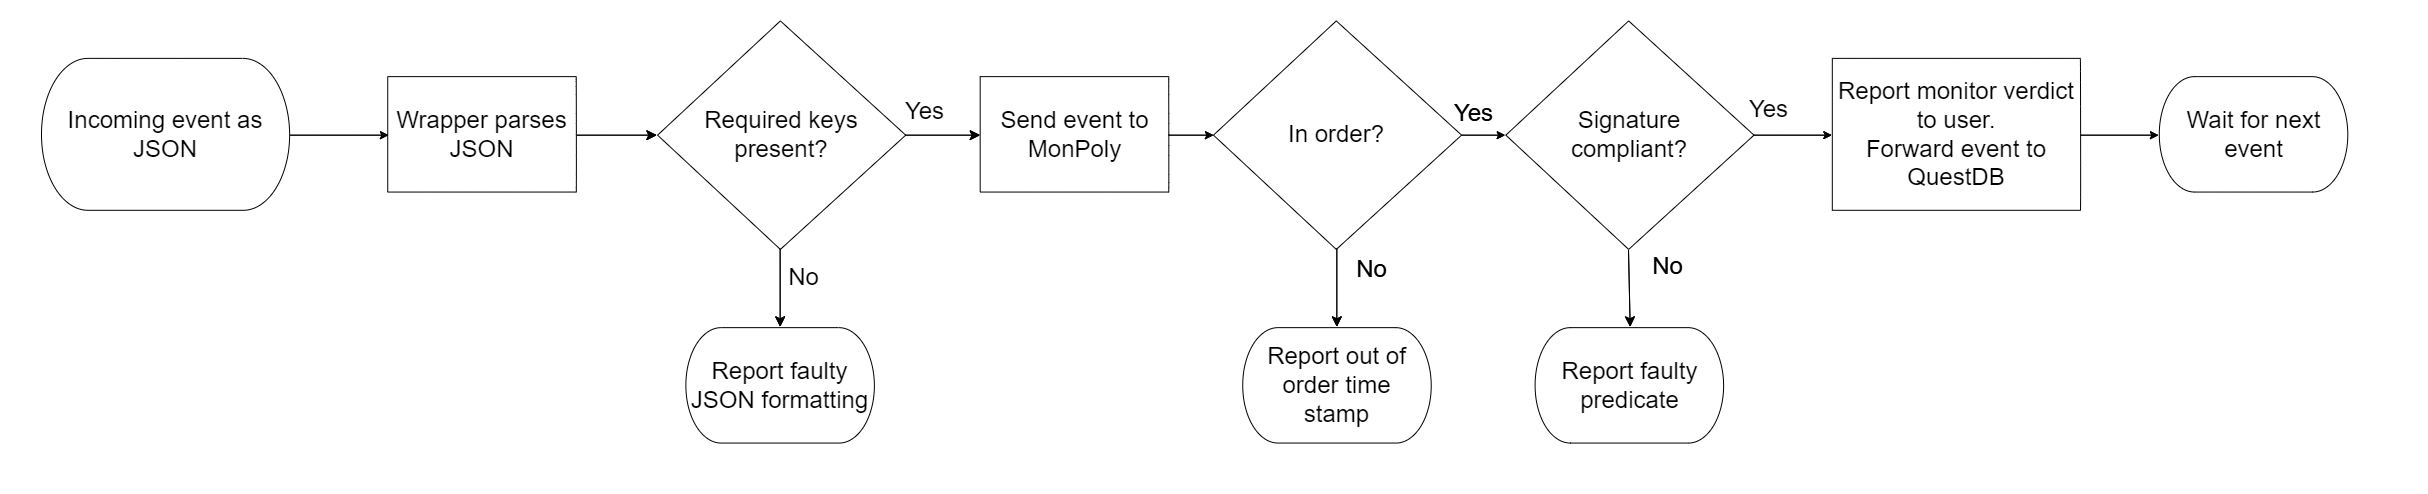
\includegraphics[width=110mm]{diagrams/flowchart.png}
    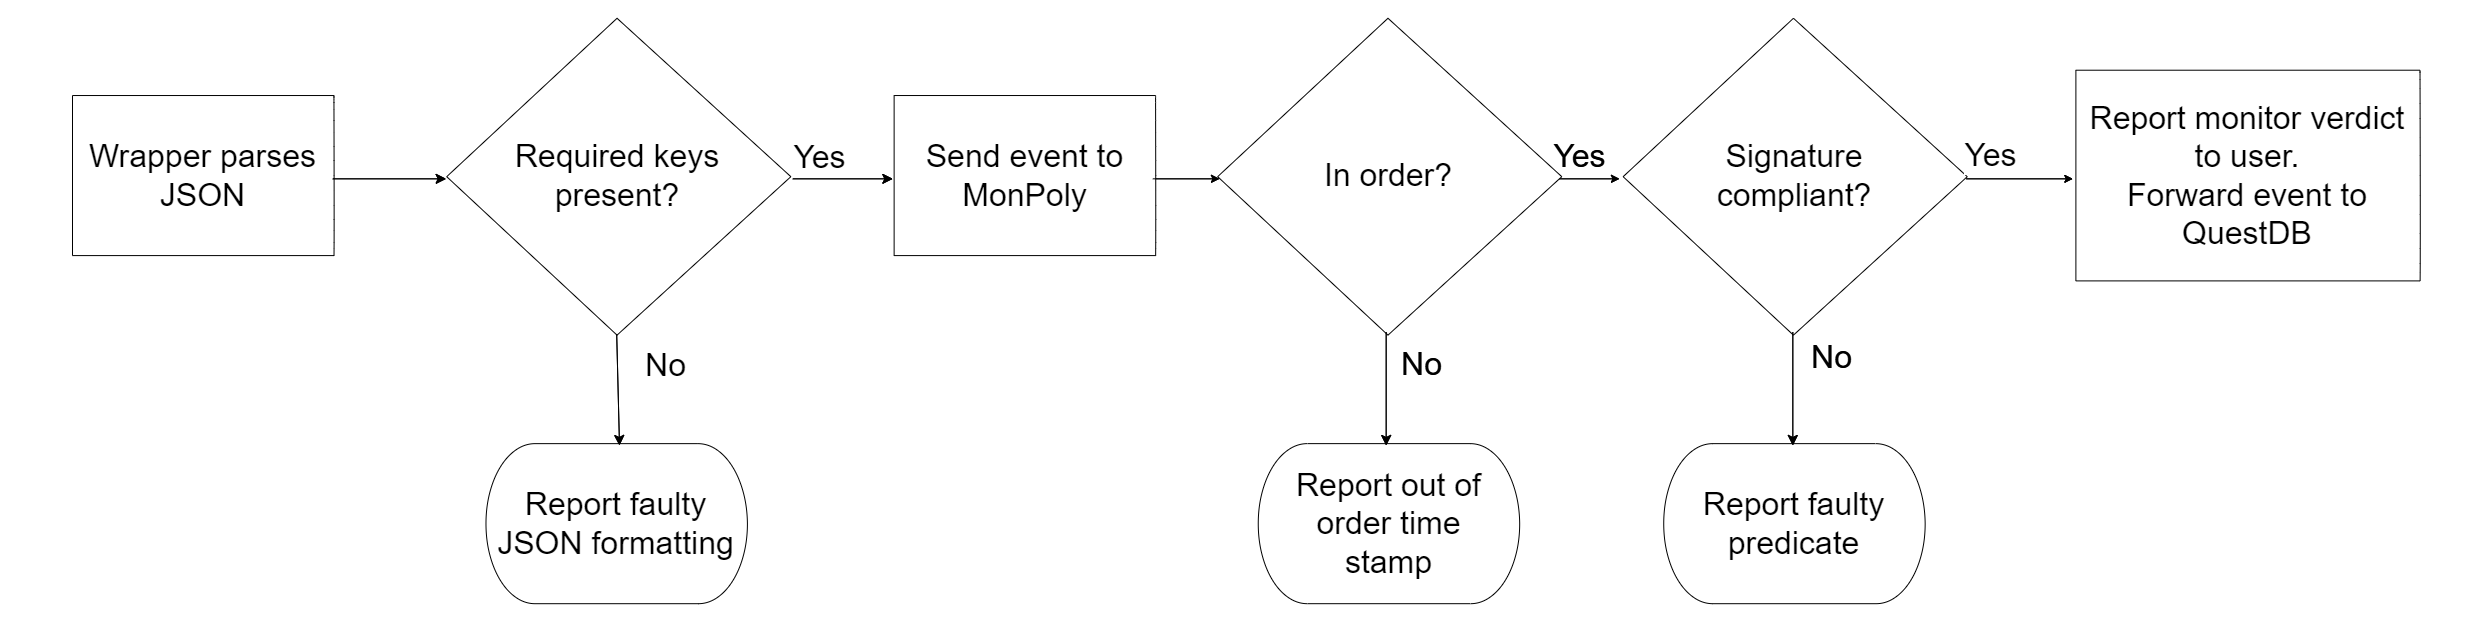
\includegraphics[width=\linewidth]{diagrams/flowchart-2.png}
    \caption{Control flow for an incoming}
\end{figure}

The naive approach to a policy change is simply reloading all events that have ever been seen by the monitor and in turn are in the database.
But we can potentially do much better than this.
An initial improvement is to only load all events in the relative interval of the new policy around the most recent time point.
We apply our idea of extended relative intervals to optimize the performance of this first version a policy change.
This version works by stopping the current MonPoly process and starting a new one.


\section{Additions to MonPoly}
We added two flags to MonPoly that, for a signature file, produce the SQL schema, as previously described, or a representation of the signature in JSON respectively.
Those flags are \texttt{-sql} and \texttt{-sig\_to\_json}.
Their usage is shown in the following example.
\begin{verbatim}
$ monpoly -sql <path/to/signature>
$ monpoly -sig_to_json <path/to/signature>
\end{verbatim}
The flag \texttt{-sql\_drop} works analogous to the \texttt{-sql} flag and produces the SQL statements for "dropping", i.e. deleting the tables in the schema.
\begin{verbatim}
$ monpoly -sql_drop <path/to/signature>
\end{verbatim}

The wrapper needs some kind of feedback when a time point has been processed, in order to return potential feedback to the user.
We added the flag \texttt{-ack\_sep} that can be added when starting to monitor a formula with MonPoly.
A separator is a semicolon.
With this flag, every time the parser reaches a semicolon, an acknowledgment gets sent to stdout.
The wrapper can thus be sure that a time point has been fully processed, and no more waiting is required.

As the wrapper does not perform any check on the names, types, and arity of predicates, we want to avoid that MonPoly exits if the wrapper sends a predicate that is "faulty" in any way.
For this purpose we have added a \texttt{-tolerate\_faulty\_predicates} flag.
This flag makes it so that any time points that contain a predicate with wrong arity and/or types of attributes, get skipped.

Next we made some additions to make MonPoly work better for our policy change method.
By default, MonPoly either runs continuously and reads input from standard input or it processes a log file and terminates once it fully processed all events in the file.
We retrieve a potentially large amount of time points from the database during a policy change.
It is useful if these events could be sent to MonPoly as a file.
But as we want to continue monitoring after processing these past time points, MonPoly cannot terminate at this point.
For this purpose we added the flag \texttt{-switch\_to\_stdin\_after\_log}.
With this flag MonPoly processes a log file and once done with that it awaits new input from standard in.
We are not necessarily interested in all the monitor verdicts of the new policy on all these past time points.
Therefore we added a flag (\texttt{-suppress\_stdout}) that suppresses any potential output while processing the time points in the log file.
The output resumes normally afterwards.

The next three flags that we added concern the relative intervals and the extended relative intervals of formulas.
They are \texttt{-get\_relative\_interval}, \texttt{-relative\_interval\_per\_predicate}, and \texttt{-relative\_interval\_per\_predicate\_json}.
The wrapper uses these commands to know which time points and events must be queried from the QuestDB upon a policy change.

\section{Performance Analysis}
For the performance evaluation of the wrapper there are essentially two angles to take.
\begin{enumerate}
    \item[RQ1]
        The first one is, how large is the overhead for monitoring a policy when using the wrapper compared to using MonPoly directly?
    \item[RQ2]
        The second point of interest is, how much can our optimizations, using extended relative intervals, improve a policy change compared to the naive approach?
\end{enumerate}

\subsection{Wrapper vs. MonPoly}
We expect the wrapper to add a certain time overhead to the monitoring as it performs the same action as MonPoly plus some more things.
We are interested in seeing how much more time these other things add to the total time.
Of course, we aim for it to be as small as possible.

To get an idea of this overhead, we measure the time that the wrapper and MonPoly alone take to process equivalent traces with the same policy and signature for both.
We ran 20 experiments with the same policy.
For every experiment we generated increasingly long traces.
In Figure \ref{fig:monpoly-wrapper-total} we present the average total time that the wrapper and MonPoly respectively took to process the events.
We can see that the wrapper takes increasingly more time, but the growth is linear.
This does not come unexpected.
A constant minimal cost will always come from running the trace through a server.
As an added measurement we sent every time point separately to MonPoly and measured the time for this.
The idea behind this is that in our implementation this is how we forward time points to MonPoly, and we wanted to get an idea how much of the overhead this might explain.
Figure \ref{fig:monpoly-wrapper-per-time-point} shows the same information, but averaged by the number of time points/ length of the trace.
One interesting observation from this graph is the different behavior of MonPoly when processing an entire log file and when receiving individual time points continuously from standard input.
For very few time points it appears that the wrapper is slightly faster than MonPoly per time point.
This probably comes down to sample size.

\begin{figure}
    \centering
    \label{fig:monpoly-wrapper-total}
    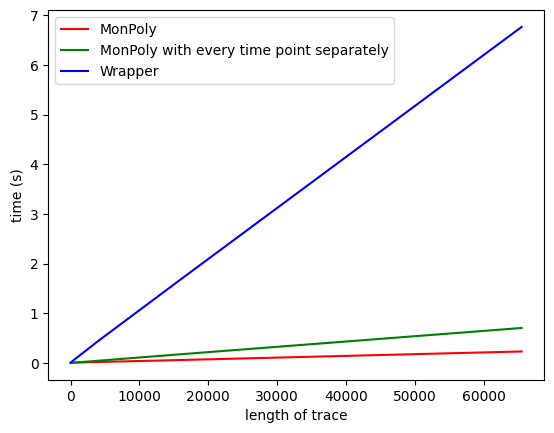
\includegraphics[width=0.8\linewidth]{diagrams/wrapper-monpoly-total.png}
    \caption{Time it takes to process variably long traces}
\end{figure}

\begin{figure}
    \centering
    \label{fig:monpoly-wrapper-per-time-point}
    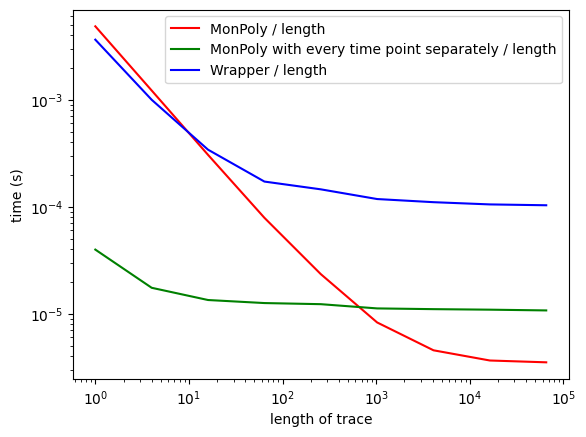
\includegraphics[width=0.8\linewidth]{diagrams/wrapper-monpoly-per-time-point.png}
    \caption{Time it takes to process a trace by the number of time points in the trace}
\end{figure}

\subsection{Policy Change Performance}

In this section we give an idea of the performance of the naive policy change where all events are in the database are processed compared to the performance with our optimization that uses only the events in the extended relative intervals (ERI).

We have compared a policy change using our optimizations to the naive approach by using two random policies and generating random traces of various lengths.
We then compare how the two methods perform for an increasing number of time points.
We have run the same randomized experiment 20 times.
The setup is that we monitor a random policy and measure the time it takes to change the policy after traces with $4^i$, for $i \in [1,9]$, time points have been stored in the database previously.
Figure \ref{fig:policy-change-total} shows the average time it takes to change the policy for both versions of a policy change in respect to the trace length.
Figure \ref{fig:policy-change-per-time-point} shows the same information, but the time has been averaged by time point.
We see that there is large variation for small traces and for a bit the naive change is actually faster, but for large traces our optimization consistently beats the baseline.
From the averaged graph we can't make out much of an improvement.
We do see that both get faster per time point, when there are more total time points.
This can potentially be attributed to amortization costs that have to be paid for a small number as well as for a large number of time points.
Of course the expected performance improvement depends heavily on the formula, if it has large extended relative intervals it is barely different from the naive case, and also on the size of the trace stored in the database.

\begin{figure}
    \centering
    \label{fig:policy-change-total}
    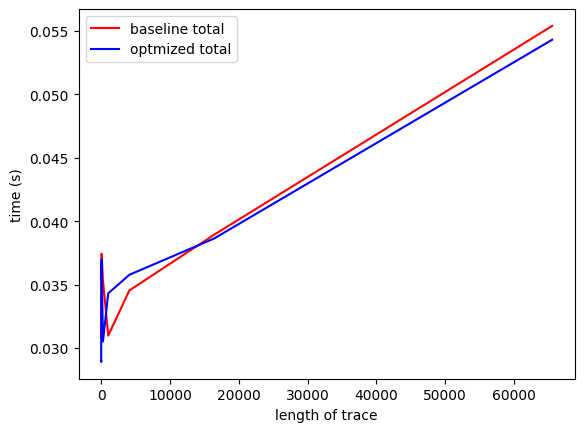
\includegraphics[width=0.8\linewidth]{diagrams/policy-change-total-time.png}
    \caption{Total time a policy change takes for various numbers of time points in a trace}
\end{figure}

\begin{figure}
    \centering
    \label{fig:policy-change-per-time-point}
    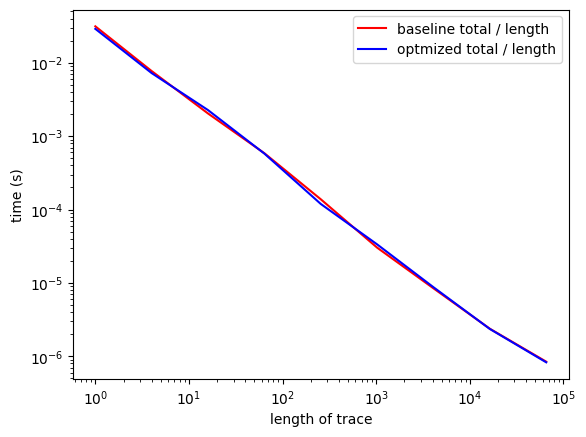
\includegraphics[width=0.8\linewidth]{diagrams/policy-change-time-per-time-point.png}
    \caption{Time it takes to change the policy in respect to the total number of events in the trace}
\end{figure}

\section{Partial Policy Change}

We have started looking into a different method for a policy change that could be done directly through MonPoly and would not rely on the wrapper and the presence of a database.
The general idea is that in many use cases it is common that a policy is made up of many individual parts and one might want to change only a small part of a formula.
Consider for example a privacy policy on a website.
Let's say a user has the ability to specify where their data may and may not be used.
Maybe they had selected very restrictive options, but now want to allow their data to be used in one specific case.
MonPoly has now continuously been monitoring the restrictive policy and also has the state for all the sub-formulas in the larger policy.
In terms of efficiency it would be useful, if the state would only need to be recomputed for the one part that got changed and if the rest of the state could be kept.

One case might be where policies are all in conjunctive normal form (CNF) and single conjuncts might get added or removed.
To remove a conjunct from the formula it needs some sort of identifier.
In a regular structure like a CNF formula this could be done by automatic indexing.
But it still poses some questions, like what happens if the monitor rewrites the formula to an equivalent one, but changes the order.
Then the user doesn't have an inherent idea of a conjuncts' location anymore.
Our solution to this problem was thus to let the user provide identifiers in the form of strings for certain sub-formulas.

We have begun implementing this change in MonPoly.
Our idea makes use of the existing commands feature that lets a user control certain aspects of MonPoly during its runtime.
We envision commands of the form "remove sub-formula x", "add formula y as a conjunct to sub-formula x".
The second example would replace place the sub formula "x and y" in place of "x".
An analogous thing for "or" with an "add disjunct" command is also perceivable.
Or also a command like "negate sub-formula x".

With all this, MonPoly would parse the new formula part, add it to the existing formula, check if the new formula is monitorable, and if so it updates the policy.
Similarly if a part gets removed a check on monitorability of the remaining formula needs to be done.
Before adding a sub-formula, the existing trace has to be checked against that sub-formula and this state must get combined with the pre-existing state of MonPoly.

We have started implementing a feature that allows for named formulas inside MonPoly.
The names should have no effect on the monitoring and solely act as the identifiers of formula parts.
For this we extended \texttt{formula} in MonPoly by an additional type, \texttt{NamedFormula of (string * formula)}.
And similarly we added the type \texttt{ENamedExtf of string * extformula * int} to \texttt{extformula}.

To specify a named (sub)formula in a MonPoly policy, we have extended the formula parser and lexer to accept formulas with the following syntax,
\begin{verbatim}
NAME[f1, name1] AND NAME[f2 OR f3, name2].
\end{verbatim}


\section{Conclusion}

\section{references}

\includepdf[pages=-]{eigenständigkeitserklärung.pdf}


\end{document}
